% !TEX root = ../../main.tex
\section{One-Class Support Vector Machine}\label{sec:one_class_svm}


%--------------------------------------------
\subsection{Support Vector Machine}\label{subsec:svm}
We will first discuss the traditional two-class \gls{svm} before we consider the one-class variant, as introduced by Cortes and Vapnik in \cite{cortes1995support}.
Consider a data set $\Omega = \{ (x_1, y_1),\allowbreak (x_2, y_2), \dots , (x_n, y_n) \}$; points $x_i \in \mathbb{R}^d$ in a (for instance two-dimensional) space where $x_i$ is the $i$-th input data point and $y_i \in \{-1, 1\}$ is the $i$-th output pattern, indicating the class membership.

A \gls{svm} can create a boundary between linear-separable data points, making it a non-probabilistic binary linear classifier.
More flexible non-linear boundaries can be obtained by the use of a non-linear function $\phi(x)$, as illustrated in Figure \ref{fig:kernel_mapping}.
This function maps the input data from space $\mathcal{I}$ to a higher dimensional space $\mathcal{F}$.
The \gls{svm} can create a linear separating hyperplane in the space $\mathcal{F}$ that separates the data points from the two classes.
When the hyperplane is projected to the (lower) original input space $\mathcal{I}$ it creates a non-linear separating curve.
This is illustrated in Figure \ref{fig:svm_mapping_spaces}.
The mapping and projection of data points can be efficient (and implicit) performed by using the kernel trick, which is discussed in section \ref{subsec:kernel_trick}.

The separating hyperplane is represented by
\begin{equation}
w^T x + b = 0,
\end{equation}
with $w \in F$ and $b \in R$.
The hyperplane that is created determines the \emph{margin} between the classes; the minimal distance from one of the data points to the hyperplane.
In geometric sense, $w$ is the normal vector indication the direction of the hyperplane and $\frac{b}{\lVert{w}\rVert}$ determines the offset of the hyperplane to the origin.
Since the distance between the two margins is equal to $\frac{2}{\lVert{w}\rVert}$, the maximum-margin hyperplane is found by minimizing $\lVert{w}\rVert$.
The data points which lie on the margin are the \emph{support vectors}.
This geometrical interpretation is illustrated in Figure \ref{fig:svm_hyperplane}.
All data points for which $y_i = -1$ are on one side of the hyperplane and all other data points (for which $y_i = 1$) are on the other side.
The minimal distance from a data point to the hyperplane is for both classes equal.
This results in a \emph{maximal margin} between the two classes.
Thus, the \gls{svm} searches for a maximal separating hyperplane.

\begin{figure}
\centering
  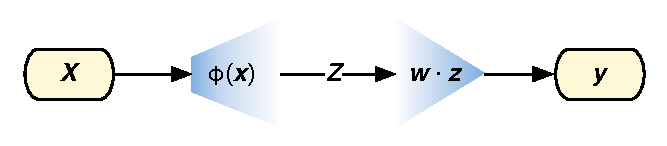
\includegraphics[width=0.5\textwidth]{./Figures/chapter3/svm_mapping_spaces.pdf}
  \caption[Mapping spaces in \gls{svm}]{The input vector $\vectorsym{x}$ from input space $\mathcal{I}$ is mapped by a non-linear function $\phi(\vectorsym{x})$ to a feature vector $\vectorsym{z}$ in the high dimensional feature space $\mathcal{F}$. The weights of $\vectorsym{w}$ create a linear separating hypeplace, which maps the high dimensional vector to the predicted outcome $\vectorsym{y}$. \TODO{Is this figure obsolete? Figure \ref{fig:kernel_mapping} shows almost the same}}
  \label{fig:svm_mapping_spaces}
\end{figure}

\begin{figure}
\centering
  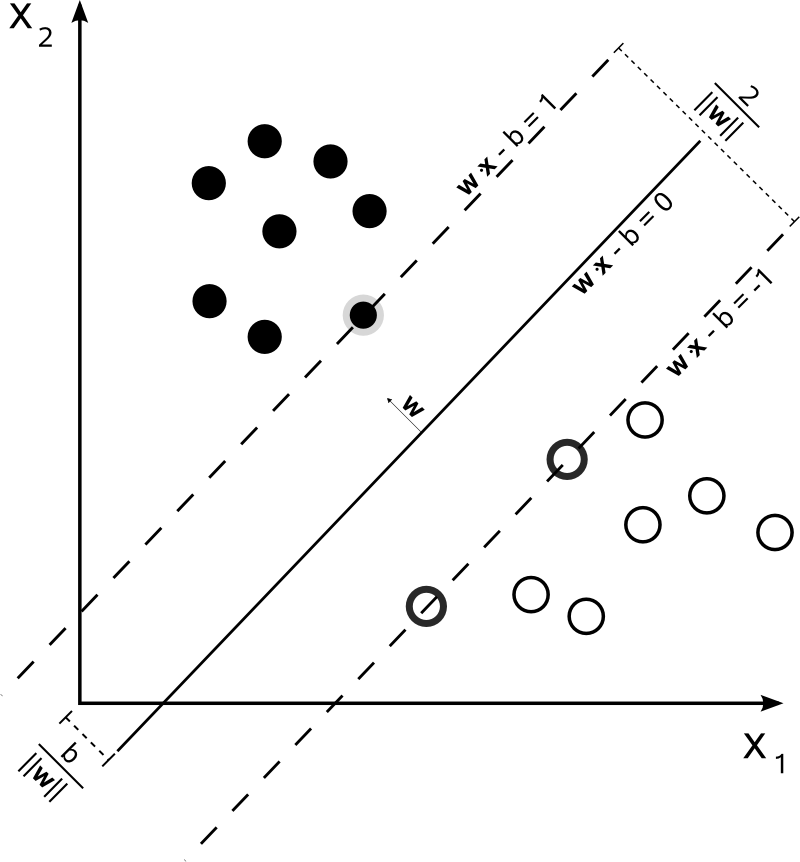
\includegraphics[width=0.5\textwidth]{./Figures/chapter3/svm_separating_plane_with_margin.png}
  \caption[\gls{svm} and the separating hyperplane]{Illustration of the separating hyperplane of a \gls{svm}. Here $w$ is the normal vector for the separating hyperplane and the distance between the two margins is $\frac{2}{\lVert{w}\rVert}$. Image from Wikipedia.org\protect\footnote}
  \label{fig:svm_hyperplane}
\end{figure}
\footnotetext{\url{http://en.wikipedia.org/wiki/File:Svm_max_sep_hyperplane_with_margin.png}}

With every classification method there is a risk of overfitting.
In that case the random error or noise of the data set is described instead of the underlying data.
The \gls{svm} classifier can use a \emph{soft margin} by allowing some data points to lie within the margin, instead of on the margin or farther away from the hyperplane.
For this it introduces \emph{slack variables} $\xi_i$ for each data point and the constant $C > 0$ the determines the trade-off between maximizing the margin and the number of data points within that margin (and thus the training errors).
The slack variables minimize the \emph{sum of deviations} rather than the \emph{number} of incorrect data points \cite{cherkassky2007learning}.
The objective function for a \gls{svm} is the following minimization function:

\begin{equation}\label{eq:svm_objective}
  \operatorname*{min}_{w,\ b,\ \xi_i} \frac{ \lVert{w}\rVert^2 }{2} + C \sum_{i=1}^n \xi_i
\end{equation}
\begin{equation}
  \begin{multlined}
  \mbox{ subject to: } \\*
  \begin{aligned}
  y_i( w^T \phi(x_i) + b) \geq & 1 - \xi_i & \mbox{ for all } i = 1, \dots, n \\*
   & \xi_i \geq 0 & \mbox{ for all } i = 1, \dots, n\\*
  \end{aligned}
  \end{multlined}
\end{equation}

\TODO{better format of above formulas. Check with notation and formulas of chapter 9 of \cite{cherkassky2007learning}.}

This minimization problem can be solved (using \gls{qp}) and transformed to its (Lagrange) dual formulation.
In the dual formulation the problem scales with the number of training examples $n$ instead of the dimensionality $d$ of the samples.
Solving this problem directly in the high dimensional feature space $\mathcal{F}$ makes it untractable.
The linear approximation function corresponds to the kernel function in the dual formulation.
Solving this dual formulation is equivalent to solving the primal formulation \cite{cherkassky2007learning}.
In the dual formulation the Lagrange multipliers $a_i >= 0$ are introduced and the decision function becomes:
\begin{equation}\label{eq:svm_lagrange}
  f(x) = \operatorname{sgn}( \sum_{i=1}^n \alpha_i y_i K(x, x_i) + b),
\end{equation}
where $K(x, x_i) = \phi(x)^T\phi(x_i)$ (which is further discussed in section \ref{subsec:kernel_trick}).
Here every data point $\mathcal{I}$ for which $a_i > 0$ is weighted in the decision function and thus ``supports'' the classification machine: hence the name ``\acrlong{svm}''.
Since it is shown that under certain circumstances \glspl{svm} show an equality to sparse representations \cite{girosi1998equivalence,smola1998connection}, there will often be relatively few Lagrange multipliers with a non-zero value.

\TODO{Add more on sparsity and good results, because of sparse representations, even in case of data of high dimensionality. e.g. \cite{cherkassky2007learning}.}

%--------------------------------------------

\subsection{Kernel trick}\label{subsec:kernel_trick}
In the previous section, \ref{subsec:svm}, the mapping function $\phi(x)$ and the kernel function $K$ were briefly mentioned.
The decision function in equation \ref{eq:svm_lagrange} only relies on the dot-products of mapped data points in the feature space $\mathcal{F}$ (\ie all pairwise distances between the data points in that space).
It shows \cite{flach2012machine} that as long as any function has the same result, without an explicit mapping to the higher dimension $\mathcal{F}$, the dot-products can be substituted by the kernel function $K$.
This is known as the \emph{kernel trick} and gives the \gls{svm} the ability to create non-linear decision function without high computational complexity.
This mapping is illustrated in Figure \ref{fig:kernel_mapping}.
Here the non-linear separating boundary in the input space $\mathcal{I}$ is mapped, via $\phi$, to a linear boundary in the feature space $\mathcal{F}$.

The kernel function $K$ can have different forms, such as linear, polynomial and sigmoidal but the most used (and flexible) form is the Gaussian \gls{rbf}.
As Smola \etal \cite{smola1998connection} state, this Gaussian kernel yields good performance, especially when no assumptions can be made about the data.
The kernel maps input space $\mathcal{I}$ to the feature space $\mathcal{F}$ which is a Hilbert Space of infinite dimensions \TODO{ref needed}:
\begin{equation}
  K(x, x') = \operatorname{exp} \left( - \frac{ \lVert x - x' \rVert ^2}{2 \sigma^2 } \right),
\end{equation}
where $\sigma \in R$ is a kernel parameter and $\lVert x - x' \rVert$ is the dissimilarity measure expressed in Euclidean distance.


\begin{figure}
\centering
  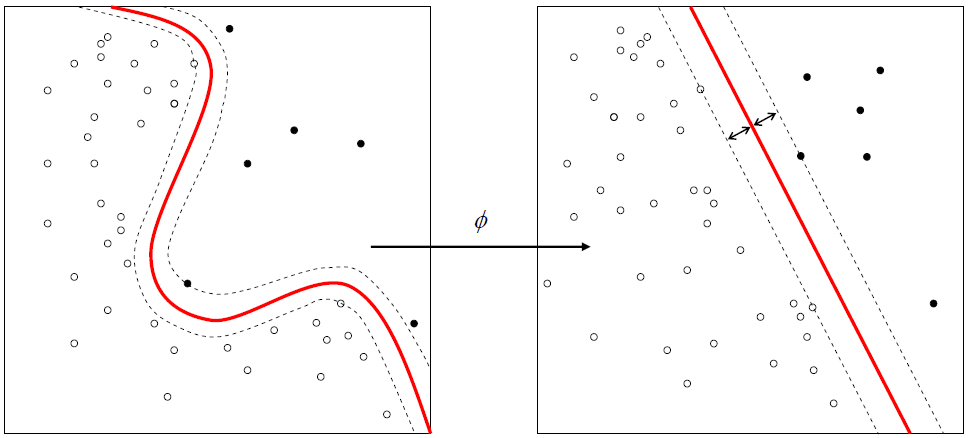
\includegraphics[width=0.8\textwidth]{./Figures/chapter3/svm_kernel_mapping.png}
  \caption[Kernel mapping]{The non-linear boundary in the input space $\mathcal{I}$ (left) is transformed to a linear boundary in the feature space $\mathcal{F}$ (right) by mapping the data points with the function $\phi$. The kernel trick uses a function $K$ which performs an implicit mapping. Image from Wikipedia.org\footnotemark}
  \label{fig:kernel_mapping}
\end{figure}
\footnotetext{\url{http://en.wikipedia.org/wiki/File:Kernel_Machine.png}}

%--------------------------------------------

\subsection{Reproducing kernel Hilbert space}
\emph{Write something on this topic? Or leave it implicit?}


%--------------------------------------------

\subsection{One-Class Support Vector Machines}\label{subsec:one-class-svm}
The classical implementation of a \gls{svm} is to classify a dataset in two distinct classes.
This is a common usecase, although sometimes there is no training data for both classes available.
Still, one would like to classify new data points as regular, or in-class, or out-of-class, \eg in the case of a novelty detection.
With that problem only data from one class is available and the objective is to recognize new data points that are not part of that class.
This unsupervised learning problem is closely related to density estimation.
In that context, the problem can be the following.
Given an underlying probabilty distribution $P$ the goal is to find a subset $S$ for which the probability that a data point from $P$ lies outside $S$ equals some predetermined value $\nu$ between $0$ and $1$ \cite{scholkopf1999support}.

We will discuss two implementations of \glspl{oc-svm}.
The first is the \gls{nu-svm} by Sch\"olkopf \etal \cite{scholkopf1999support} and closely follows the above problem statement regarding density estimation.
The second, on which we will base our change detection method, is the \gls{svdd} by Tax and Duin \cite{tax1999support}.

\TODO{Add something about robustness, discusses in section 9.2 from \cite{cherkassky2007learning,chen2004m}}

%--------------------------------------------

\subsection{\acrlong{nu-svm}}\label{subsec:nu-svm}
The first of the \gls{oc-svm} methods we will discuss is often referred to as \gls{nu-svm} and introduced by Sch\"olkopf \etal \cite{scholkopf1999support}.
Instead of estimating the density function of an distribution $P$, it focuses on an easier problem: the algorithm find regions in the input where the ``probability density lives''.
This results in a function such that most of the data is in the region where the function is nonzero.

The constructed decision function $\mathcal{F}$ resembles the function discussed in Section \ref{subsec:svm}.
It returns the value $+1$ in a (possibly small) region capturing most of the data points, and $-1$ elsewhere.
The method maps the data points from input space $\mathcal{I}$ to a feature space $\mathcal{F}$ (following classical \glspl{svm}).
In that space $\mathcal{F}$ it separates the data points with maximal margin from the origin, with a hyperplane.
For a new data points $x$, the function value $f(x)$ determines wheter the data point is part of the distribution (\ie the value is $+1$) or a novelty (\ie the value is $-1$).
The hyperplane is represented by $g(x) = w \cdot \phi(x) + \rho = 0$ and the decision function is $f(x) = \operatorname{sgn}(g(x))$.
This hyperplane and the separation from the origin is illustrated in Figure \ref{fig:nu-svm}.

\begin{figure}
  \centering
    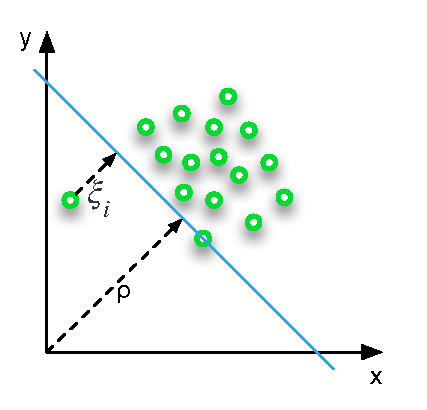
\includegraphics[width=0.5\textwidth,keepaspectratio]{./Figures/chapter3/nu-svm.pdf}
  \caption[\gls{nu-svm}]{Graphical representation of \gls{nu-svm}. The separating hyperplane $w \cdot \phi(x_i) + \rho = 0$ create a maximal margin, in the feature space, between the data points and the origin. Slack variables $\xi_i$ are used to create a soft margin.}
  \label{fig:nu-svm}
\end{figure}

The objective function to find the separating hyperplane is the following minimization function, which can be solved using \gls{qp}:

\begin{equation}\label{eq:nu-svm_objective}
  \operatorname*{min}_{w,\ \xi_i,\ \rho } \frac{\lVert w \rVert ^2}{2} + \frac{1}{\nu n} \sum_{i=1}^n \xi_i - \rho
\end{equation}
\begin{equation}
  \begin{multlined}
    \mbox{ subject to: } \\
    \begin{aligned}
      (w \cdot \phi(x_i)) \geq & \rho - \xi_i & \mbox{ for all } i = 1, \dots, n \\
      & \xi_i \geq 0 & \mbox{ for all } i = 1, \dots, n \\
    \end{aligned}
  \end{multlined}
\end{equation}

The decision function in the dual formulation with Lagrange multipliers is denoted as:
\begin{equation}\label{eq:nu-svm_lagrange}
f(x) = \operatorname{sgn}((w \cdot \phi(x_i)) - \rho) = \operatorname{sgn}( \sum_{i=1}^n \alpha_i K(x, x_i) - \rho)
\end{equation}

In the classical \gls{svm} objective function, as denoted in Equation \ref{eq:svm_objective}, the parameter $C$ decided the smoothness of the boundary, with respect to the slack variables $\xi_i$.
In the formulation of \gls{nu-svm} the equivalent parameter is $\nu \in (0,1)$ (hence the name).
It characterizes the solution in two ways:
\begin{enumerate}
  \item $\nu$ is an upper bound on the fraction of outliers, \ie training examples regarded as out-of-class.
  \item $\nu$ is a lower bound on the fraction of \glspl{sv}, \ie training examples with a nonzero Lagrange multiplier $\alpha_i$.
\end{enumerate}
When $\nu$ approaches $0$, the penalty factor for nonzero Lagrange multipliers ($\frac{1}{\nu n}$) becomes infinite, and thus the solution resembles a \emph{hard margin} boundary.

This method creates a \emph{hyperplane}, characterized by $w$ and $\rho$, that separates the data with maximal margin from the origin in the feature space $\mathcal{F}$.
In the following section we will discuss an alternative method, which uses an circumscribing \emph{hypersphere} to characterize the data (and the region of distribution $P$ where the density (or: support) lives).


%--------------------------------------------

\subsection{\acrlong{svdd}}\label{subsec:oc-svm-svdd}
The method introduced by Tax and Duin \cite{tax1999support}, known as \acrlong{svdd}, takes a spherical instead of planar approach.
The boundary, created in feature space $\mathcal{F}$, forms a hypersphere around the (high density region of the) data.
The volume of this hypersphere is minimized to get the smallest enclosing boundary.
The chance of accepting outlier objects is thereby also minimized \cite{tax2003online}.
By allowing outliers using slacks variables, in the same manner as classical \gls{svm} and \gls{nu-svm}, a soft margin is constructed.

\begin{figure}
  \centering
    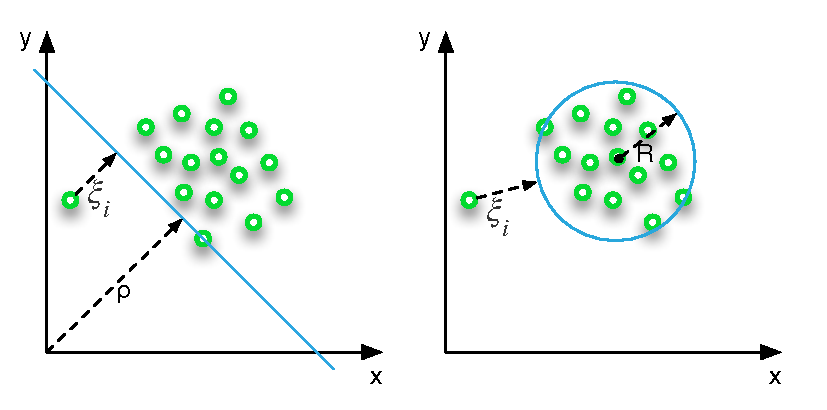
\includegraphics[width=0.5\textwidth,keepaspectratio]{./Figures/chapter3/nu-vs-svdd.pdf}
  \caption[Difference \gls{nu-svm} and \gls{svdd}]{Graphical representation of the difference between \gls{nu-svm} (left) and \gls{svdd} (right). Note that for the sake of simplicity the kernel functions are not applied.}
  \label{fig:nu-vs-svdd}
\end{figure}

The constructed hypersphere is characterized by a center $\mathbf{a}$ and a radius $R > 0$ as distance from the center to (any data point that is a \gls{sv} on) the boundary, for which the volume, and thus the radius $R$, will be minimized.
The center $\mathbf{a}$ is a linear combination of of the support vectors.
Like the classical \gls{svm} and \gls{svdd} it can be required that all the distances from the data points $x_i$ to the center $\mathbf{a}$ are strict less then $R$ (or equivalent measure, to create a hard margin) or soft margins are allowed by using slack variables $\xi_i$.
In the case of a soft margin, the penalty is determined by $C$ and the minimization is expressed as Equation \ref{eq:svdd_objective}.
This principle is illustrated in the right image or Figure \ref{fig:nu-vs-svdd}.
Instead of a separating hyperplane, constructed by \gls{nu-svm} and illustrated on the left of the Figure, the \gls{svdd} creates a hypersphere (in the illustration a cricle) around the data points.
By using kernel functions (\eg the \gls{rbf}) the hyperspheres in the high dimensional feature space $\mathcal{F}$ corresponds to a flexible and tight enclosing boundary in input space $\mathcal{I}$.
Possible resulting closed boundaries are illustrated in Figure \ref{fig:svdd-boundary}.
This enclosing boundary is obtained by minimizing the following error function $L$ which contains the volume of the hypersphere and the distance from the boundary to the outlier objects:
\begin{equation}\label{eq:svdd_objective}
  L(R, \vectorsym{a}, \vectorsym{\xi}) = R^2 + C \sum_{i=1}^n \xi_i
\end{equation}
\begin{equation}
  \begin{multlined}
    \mbox{ subject to: } \\
    \begin{aligned}
      \lVert x_i - \mathbf{a} \rVert ^ 2 \leq & R^2 + \xi_i & \mbox{ for all } i = 1, \dots, n \\
      & \xi_i \geq 0 & \mbox{ for all } i = 1, \dots, n \\
    \end{aligned}
  \end{multlined}
\end{equation}
In the dual Lagrangian formulation of this error function $L$ the multipliers $\vectorsym{\alpha}$ are maximized:
\begin{equation}\label{eq:svdd_lagrange}
  L = \sum_{i} \alpha_i(x_i \cdot x_i) - \sum_{i,j} \alpha_i \alpha_j(x_i \cdot x_j)
\end{equation}
\begin{equation}
  \begin{multlined}
    \mbox{ subject to: } \\
    \begin{aligned}
    0 \le \alpha_i \le C, \sum_{i} \alpha_i = 1
    \end{aligned}
  \end{multlined}
\end{equation}

In the maximization of Equation \ref{eq:svdd_lagrange} a large fraction of the multipliers $\alpha_i$ become zero and for a small fraction $\alpha_i > 0$.
This small fraction, for which $\alpha_i$ is non-zero, are called the \glspl{sv} and these objects lie on the boundary of the description.
The center of the hypersphere only depends on this small number of \glspl{sv} and the objects for which $\alpha_i = 0$ can be disregarded from the solution.
Testing the membership of a (new) object $\vectorsym{z}$ is done by determining if the distance to the center $\vectorsym{a}$ of the sphere is equal or smaller to the radius $R$:
\begin{equation}\label{eq:svdd_test_object}
  \lVert \vectorsym{z} - \vectorsym{a} \rVert ^2 = (\vectorsym{z} \cdot \vectorsym{z}) - 2 \sum_{i} \alpha_i(\vectorsym{z} \cdot \vectorsym{x}_i) + \sum_{i,j}(\vectorsym{x}_i \cdot \vectorsym{x}_j) \le R^2
\end{equation}

\TODO{Note of inner products and that it can be replaced by kernel functions. Good ref: page 4/158 from \cite{tax2002uniform} and \cite{tax1999support}.}

Because the Gaussian \gls{rbf} often yields good (\ie tight) boundaries, this set of kernels fuctions is commonly used:
\begin{equation}
  (\vectorsym{x} \cdot \vectorsym{y}) \rightarrow K(\vectorsym{x},\vectorsym{y}) = \operatorname{exp}\left(- \frac{\lVert \vectorsym{x} - \vectorsym{y} \rVert ^2}{\sigma^2}\right)
\end{equation}
Using this kernel function, the Lagrangian error function $L$ of Equation \ref{eq:svdd_lagrange} changes to:
\begin{equation}\label{eq:svdd_lagrange_kernel}
  L = 1 - \sum_{i} \alpha_i^2 - \sum_{i \ne j} \alpha_i \alpha_j K(x_i, x_j)
\end{equation}
Using Equation \ref{eq:svdd_test_object}, the following kernel formulation needs to hold for a new object $\vectorsym{z}$ to lie within the hypersphere:
\begin{equation}\label{eq:svdd_inequality}
  \sum_{i} \alpha_i K(\vectorsym{z}, x_i) \le \frac{1}{2} \left( 1 - R + \sum_{i,j} \alpha_i \alpha_j K(x_i, x_j) \right)
\end{equation}

\begin{figure}
  \centering
    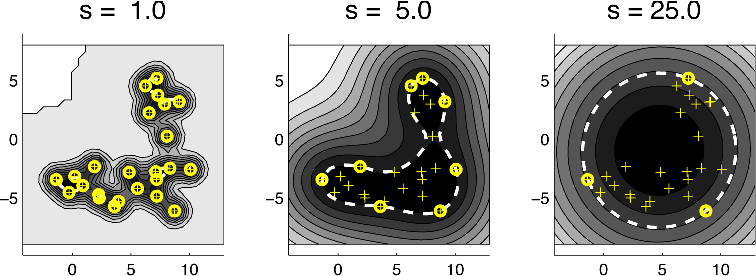
\includegraphics[width=0.5\textwidth,keepaspectratio]{./Figures/chapter3/svdd-boundary.pdf}
  \caption[\gls{svdd} boundary]{The \gls{svdd} method trained on a banana-shaped data set with different sigma-values for the \gls{rbf} kernel. Solid circles are support vectors, the dashed line is the boundary. Image by Tax \cite{tax2001one}.}
  \label{fig:svdd-boundary}
\end{figure}

\begin{figure}
  \centering
    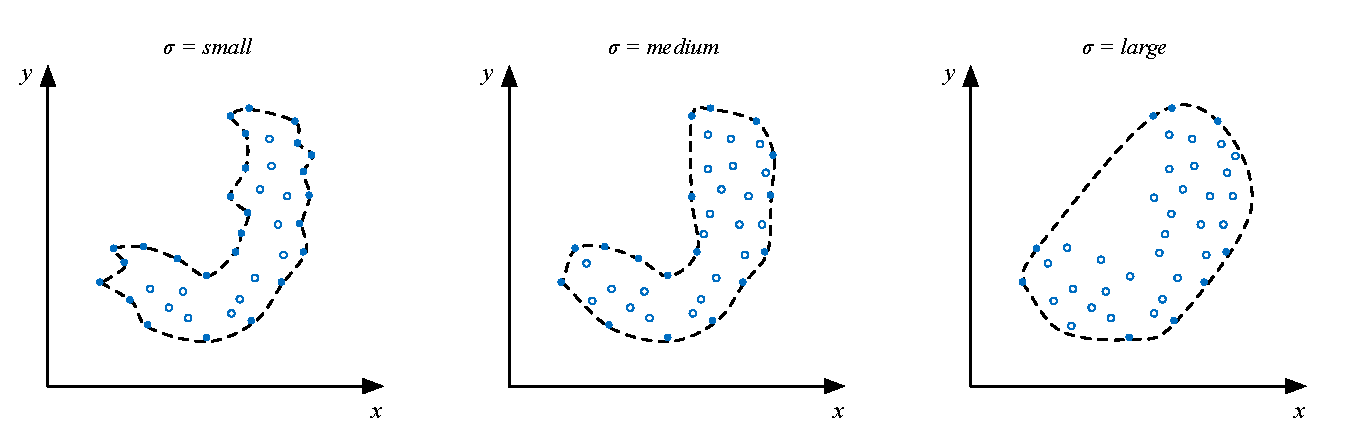
\includegraphics[width=0.8\textwidth,keepaspectratio]{./Figures/chapter3/svdd-parameter-sigma.pdf}
  \caption[\gls{svdd} boundary]{The \gls{svdd} method trained on a banana-shaped data set with different $\sigma$-values for the \gls{rbf} kernel. Solid circles are support vectors, the dashed line is the boundary.}
  \label{fig:svdd-boundary-sigma}
\end{figure}

\TODO{Use Figure \ref{fig:svdd-boundary} or \ref{fig:svdd-boundary-sigma}?}

\TODO{Note that \gls{svdd} and \gls{nu-svm} have identical solutions when data is preprocessed to have unit form (in the case of \gls{nu-svm}) \cite{tax2002uniform}.}

%--------------------------------------------
\subsection{Kernel Function}\label{subsec:kernel_function}

\begin{itemize}
  \item Explain RBF kernel
  \item Explain RKHS? (Hilbert Space)
\end{itemize}

A common class for kernel function is the \acrlong{rbf}.
These function are of the form
\begin{equation}
  g(x) = \operatorname*{sign} \left(  \sum_{i=1}^{n} \alpha_i \operatorname*{exp} \left\{ \frac{|\vectorsym{x} - \vectorsym{x}_i|^2}{\sigma^2} \right\} \right),
\end{equation}
where $\sigma$ defines the width.
The inner product kernel is of the form
\begin{equation}
  K(\vectorsym{x}, \vectorsym{x}') = \operatorname*{exp} \left\{ - \frac{| \vectorsym{x} - \vectorsym{x}'|^2}{\sigma^2} \right\}.
\end{equation}

Note that with the \gls{rbf} class of kernel functions the number of basis functions, the center parameters that correspond to the support vectors, and the weights in the output layer are all automatically determined via the optimal hyperplane \cite{cherkassky2007learning}.
The width parameter $\sigma$ is equal for all basis functions and is set a priori and determines the flexibility and complexity of the boundary.
In Section \ref{subsec:svm_model_parameters} this (hyper)parameter for a \gls{svm} is further discussed.
Other examples of kernel function classes are \emph{pylonomial functions} of degree $q$, \emph{neural networks}, \emph{splines} of order $m$ with $b$ nodes, and \emph{Fourier expansions}.
\TODO{More on basis functions. \cite{cherkassky2007learning}, chapter 9.4}

-- Quotes and refs to use --
$k(\mathbf{x}_i, \mathbf{x})$ is a kernel function computing a dot product in feature space, introduced by Aizerman \etal \cite{aizerman1964theoretical}.
``Training a \gls{svm} with Gaussian \gls{rbf} kernels corresponds to minimizing the specific cost function with a regularization operator'' \cite{smola1998connection}. \\

``Gaussian kernels tend to yield good performance under general smoothness assumptions and should be considered especially of no additional knowledge of the data is available.'' \cite{smola1998connection}. \\

``Choosing a small width of the kernels leads to high generalization error as it effectively decouples the separate basis functions of the kernel expansion into very localized functions which is equivalent to memorizing the data, whereas a wide kernel tends to oversmooth.'' \cite{smola1998connection}. \\

``For small values of $\sigma$ almost all $\alpha_i >0$ and the \gls{svdd} resembles a Parzen density estimation.'' \cite{tax2002uniform} page 4, \cite{tax1999support} page 4. \\

sparsity, RKHS: \cite{girosi1998equivalence} \\

Kernels for Support Vector Classifiers where first (?) used by Vapnik \cite{vapnik1998statistical}.



%--------------------------------------------

\subsection{SVM model parameters}\label{subsec:svm_model_parameters}
\gls{svm}-model selectiong and tuning depends on two type of parameters \cite{cherkassky2007learning}:
\begin{enumerate}
  \item Parameters controlling the `margin' size,
  \item Model parameterization, \eg the kernel type and complexity parameters.
  For the \gls{rbf} kernel the width parameter determines the model complexity.
\end{enumerate}

In case of a \gls{rbf} kernel, the width parameter $\sigma$ determines the flexibility and complexity of the boundary.
The value of this parameter greatly determines the outcomes of the algorithm (\eg \gls{svdd}) as illustrated in Figure \ref{fig:svdd-boundary}.
With a small value for the kernel width $\sigma$, each data point will tend to be used as a support vector (for almost all $\alpha_i > 0$) and the \gls{svdd} solution resembles a Parzen density estimation.
For large values of $\sigma$, the solution will resemble the original hypersphere solution is obtained (in contrast with a tight boundary around the data).
With a large value for the width $\sigma$, the boudary approximates the spherical boundary.

\TODO{More on SVM parameters, \cite{cherkassky2007learning}, section 9.8, page 446}

\TODO{Analysis of C/$\nu$-parameter, which sets a lower bound for the fraction of support vectors and an uppor bound for samples that will be outliers. \cite{flach2012machine} section 9.8 and \cite{scholkopf2002learning} and other Sch\"olkopf material.}

\TODO{Maybe add section about ``Change indication'' rather than ``detection''?}

-- Notes --
\begin{itemize}
  \item Low target rejection rate $f_{T-}$ and low outlier acceptance rate $f_{O+}$. When only target examples are present, the first one can be estimated by the number of support vectors that we obtain as a solution of Lagrangian \ref{eq:svdd_lagrange_kernel}.
\end{itemize}

-- Literature --

\TODO{These papers need to be referenced and included}

``A geometric approach to support vector machine (SVM) classification'' \cite{mavroforakis2006geometric}. 136, 2006 \\

``Least squares one-class support vector machine'' \cite{choi2009least}. 27, 2009 \\

``On simple one-class classification methods'' \cite{noumir2012simple}. 2012  --> decouples radius and center optimization, gives fast approximations instead of precise results. \\